\documentclass[%
 reprint,
 amsmath,amssymb,
 aip,
]{revtex4-1}

\usepackage{graphicx}% Include figure files
\usepackage{dcolumn}% Align table columns on decimal point
\usepackage{bm}% bold math
\usepackage{hyperref}% add hypertext capabilities

\preprint{APS/123-QED}
\begin{document}
\title{Acoustics I project: rotating and resonant waves in a cylindrical cavity}
\author{Mathieu Maréchal\\ Supervisor: Guillaume Penelet}
\affiliation{
    M1 Wave Physics \& Acoustics\\Le Mans Université
}%
\date{\today}

\begin{abstract}
    \textbf{Abstract:} abstract abstract abstract abstract abstract abstract abstract abstract abstract abstract abstract abstract abstract abstract abstract abstract abstract abstract abstract abstract abstract abstract abstract abstract abstract abstract abstract abstract abstract abstract abstract abstract abstract abstract abstract abstract abstract abstract abstract abstract abstract abstract abstract abstract abstract abstract abstract abstract abstract abstract abstract abstract abstract abstract abstract abstract abstract abstract abstract abstract abstract abstract abstract abstract abstract.
\end{abstract}

\maketitle
\section{Introduction}
Cylindrical waveguides and modal analysis are among the key notions tackled in the Acoustics I class. And what better way to make use of these two notions than to study rotating waves. This present paper describes the project led within the framework of this course, dealing with resonant and rotating waves in a cylindrical resonant cavity. Rotating waves are not a very hot topoc within the acoustics research topics, they are more dealt with for quantum and electromagnetic waves. However, they were studied by Ceperley \cite{ceperley2002} who introduces rotating waves for water and for acoustics. One interesting aspect to this type of wave is that it transfers its angular momentum to matter as studied by \emph{Santillan et al.} \cite{santillan2009}. What follows will focus on the ways to generate an acoustic vortex or in other words, a rotating wave field. This study will be done in several parts. Firstly, one has to study analytically the characteristics of the considered cylindrical cavity, and in particular its nodal lines for specific modes, along which the point sources generating the rotating field will be placed. Then, making use of the superposition principle, one will be able to numerically simulate several phase-shifted sources exciting the cavity. Finally, controlling the phasing of these sources, one should be able to control the nature of the wave propagating in the cavity, thus allowing the production of a vortical wave field. 

\section{Investigating the nodal lines of the cylindrical cavity using a single point source}

Let a rigid cylinder of radius $R$ and length $d$ containing air, with density $\rho_0$ and sound celerity $c_0$. There is a point source inside of the cylinder creating an acoustic field $\tilde{p}(\vec{r}, t)$, where $\vec{r} = (r, \theta, z)$ located at $\vec{r}_0 = (r_0, \theta_0, z_0)$. This equation satisfies the Helmholtz equation

The system considered in this paper is a cylinder which includes one (and thereafter several) loudspeaker at $(r_0, \theta_0)$ on its upper wall. This point source imposes a driving force $q_0$ oscillating at a $\omega$ frequency. The cylinder is filled with air, a lossless medium with density $\rho_0 = 1.2$ kg.m$^3$ and sound celerity $c_0 = 343$ m/s. A representation of the studied system is proposed in figure \ref{fig:schema}. The edges of the cavity are all considered rigid, thus giving the following boundary conditions on the acoustic field
\begin{equation}
   \begin{split}
       \tilde{p}(r, \theta + 2 \pi , z) &= \tilde{p}(r, \theta, z),\\
       \left. \tilde{v}_z \right|_{z=0} & = \left. \tilde{v}_z \right|_{z=d} = 0,\\
               \left. \tilde{v}_r \right|_{r=R} & = 0 \Rightarrow J'_m (k_{mn}R) = 0.
   \end{split} 
\end{equation}
Due to the periodicity condition, we have that the clockwise and anticlockwise spinning modes $m \in \mathbb{Z}$ are integers. Furthermore, due to the Bessel functions properties stating that $J_m = (-1)^m J_{-m}$ the same order symmetric modes $m$ and $-m$ are eigenpairs and share the same eigenvalues \cite{rona2007}, so that $m \in \mathbb{N}$.

\subsection{Modal expansion in the two-dimensional case}
During this part, a 2D pressure field $\tilde{p}(r, \theta)$ will be considered: it will only depend on its azimuthal $\theta$ and radial $r$ coordinates. The wave equation to solve in the cavity is inhomogenenous,
\begin{equation}
    \begin{split}
        \frac{\partial \tilde{p}^2}{\partial r^2} + \frac{1}{r} \frac{\partial \tilde{p}}{\partial r} &+ \frac{1}{r^2} \frac{\partial \tilde{p}^2}{\partial \theta^2} + k^2 \tilde{p}\\ &= -i \omega q_0 \delta(r - r_0) \delta(\theta - \theta_0),
    \end{split}
\end{equation}
with $k = \omega/c_0$ being the wavenumber and $\delta$ is the Dirac-Delta distribution. The solution of the field will be stated by making use of a modal analysis, which can be generally written as 
\begin{equation}
    \tilde{p}(r, \theta) = \sum_{m,n} \tilde{A}_{mn} \Psi_{mn}.
\end{equation}
Using $\Psi_{mn} = J_m (k_{mn}r)\left[ \tilde{A}_{\theta m} \cos(m \theta) + \tilde{B}_{\theta m} \sin(m \theta) \right]$ as the eigenfunction, we will be able to find the amplitude expression. Next, one has to orthogonalize each part of the eigenfunction using successive scalar products $\langle \Psi_{mn} | \Psi_{m'n} \rangle = \int_a^b  \Psi_{mn}\Psi_{m'n} dx $ on the cosine term, sine term and finally the Bessel function, with respectively $\frac{1}{2\pi}\int_0^{2\pi}(\ldots)\cos(m'\theta) d\theta$, $\frac{1}{2\pi}\int_0^{2\pi}(\ldots)\sin(m'\theta) d\theta$, and $\int_0^R r (\ldots) J_m(k_{mn}r)dr$. These operations will allow us to determine the expression of the modal expansion of the pressure field.\\



\begin{figure}
    \centering
    \includegraphics[width=.35\textwidth]{figures/schema.pdf}
    \caption{Representation of the cylindrical cavity of radius $R$ and height $d$ with one point source at $(r_0, \theta_0)$}
    \label{fig:schema}
\end{figure}

Applying the two scalar products on the trigonometric function terms yields the following unified result for the problem as stated in the project guidelines \cite{guidelines}
\begin{equation}
    \begin{split}
    \sum_n \left[ k^2 - k_{mn}^2 \right] &\frac{\tilde{A}_{mn}}{2 - \delta_m^0} J_m(k_{mn}r)\\=& - i \omega q_0 \delta(r - r_0) \sin(m\theta_0)
    \end{split} \label{eq:unifres}
\end{equation}

Thereafter, the inner product to imply orthogonality on the Bessel function $J_m (k_{mn} r)$ involves, if $n = n'$,
\begin{equation}
    \begin{split}
        \int_0^R r& J_m (k_{mn} r) J_m (k_{mn'} r) dr\\ &= \frac{k^2_{mn} R^2 - m^2}{2 k^2_{mn}} J^2_m (k_{mn} R).    \end{split} \label{eq:dotbesselres}
\end{equation}
This equation is 0 in the case $n \ne n'$. Finally, applying equation (\ref{eq:dotbesselres}) on (\ref{eq:unifres}) gives the expression of the amplitude term
\begin{equation}
    \tilde{A}_{mn} = \frac{2 - \delta_m^0}{k^2_{mn} - k^2} i \omega q_0 \Psi_{m}(r_0).
\end{equation}

This expression is applicable for $m \ne 0$, otherwise the Kronecker delta term $\delta_m^0 = 0$. Thus, the expression for this part of the global expression will be taken out of the sum and expressed as its own; the sum $\sum_{m, n}^{\infty}$ will instead start at $m = 1$, $\sum_{m=1, n=0}^{\infty}$

The pressure field expression has the following form 
\begin{equation}
    \tilde{p}(r, \theta) = \sum_{m,n} \tilde{A}_{mn} J_m(k_{mn}r)\cos(m \theta)
\end{equation}

The solution of the pressure field for the 2D case is 
\begin{equation}
   \begin{split}
       \tilde{p}(r, \theta) =& \frac{2 i \omega q_0 r_0}{R^2} \sin(m\theta_0) \bigg[ \frac{1}{k^2} + \sum_{m=1,n}^{\infty} \frac{2}{k^2_{mn} - k^2} \frac{J_m (k_{mn} r_0)}{J^2_m(k_{mn}R)}\\ &\times \left(1 - \cfrac{m^2}{k^2_{mn}R^2}\right)^{-1} J_m(k_{mn}r)\cos(m \theta) \bigg] 
   \end{split} 
\end{equation}

\subsection{Modes of the cavity}
Now that the pressure field expression was derived, one can make use of this analytical solution to plot the resonance modes of the cylindrical cavity. A figure can be constituted for a range of modes $mn$ from 10 to 32, and is presented in figure \ref{fig:modes}.

\begin{figure*}
    \centering
    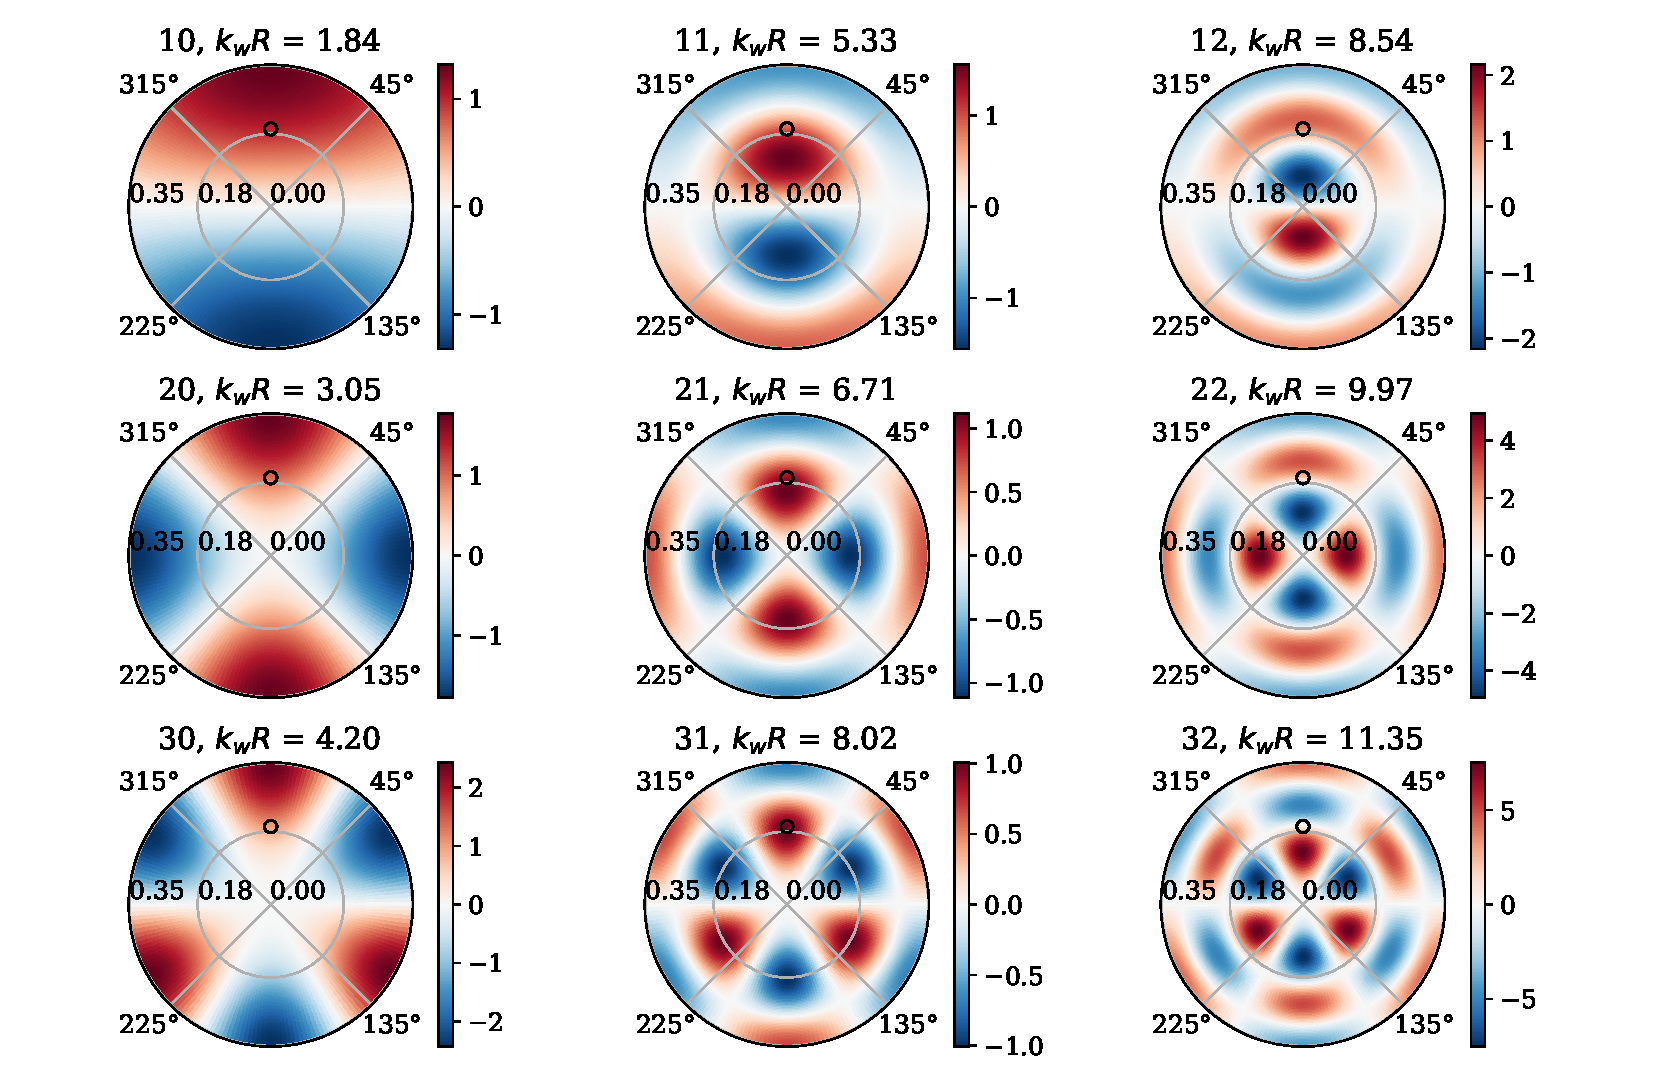
\includegraphics[width=\textwidth]{figures/modes.png}
    \caption{Modes $mn$ of the cavity generated by a single point source, represented by a black circle and located at ($r_0$ = 0.192m, $\theta_0$ = 0$^\circ$), emitting a flow $q_0 = 10^{-6}$ m$^3$/s. The real pressure field is represented, normalized with respect to the pressure at the point source. The values of $k_w R$ displayed are the values for which $J'_m$ is 0, at the given mode.}
    \label{fig:modes}
\end{figure*}

One way of studying and trying to observe rotational waves would be to put our considered sources along nodal lines: if one uses for example the nodal lines for the 11 mode, it's quite easy as one nodal line has a circular shape along the cylinder edge, at around $r = 0.25$ m.

\begin{figure}
    \centering
    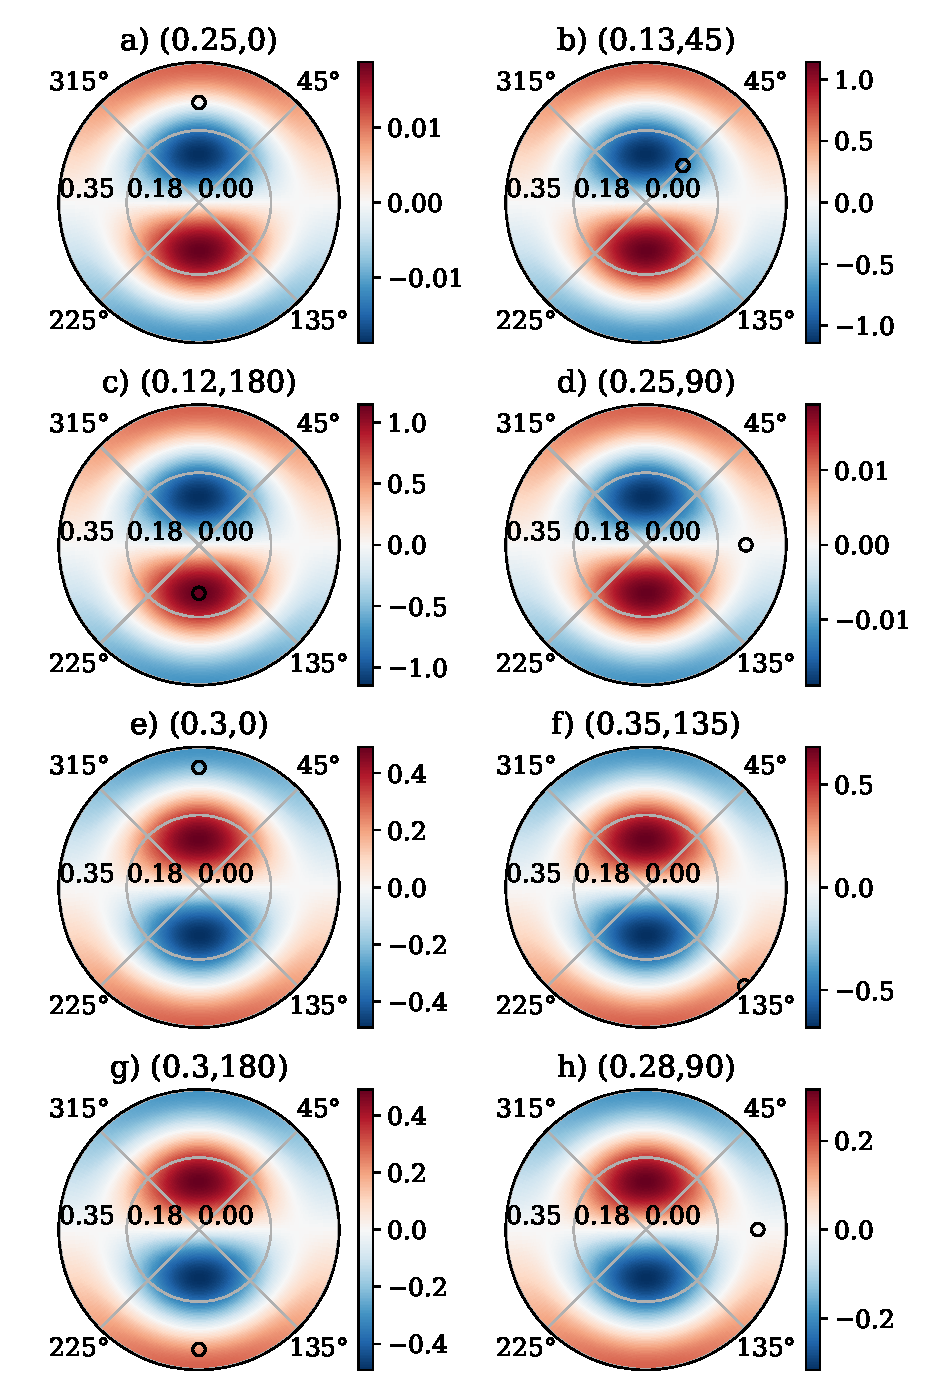
\includegraphics[width=0.45\textwidth]{figures/source_pos.png}
    \caption{Investigation of the source position on the pressure field: amplitude and phase evolution in the 11 mode. When the source is set at a coordinate r after the central nodal line, the field gets inverted}
    \label{fig:source_pos}
\end{figure}

\subsection{Extension to 3D}
\textbf{Nouvelle façon de procéder}

The source term $q^{\star} = -i \omega q_0$. The wavenumber is
\begin{equation}
    k^2 = k_{mn}^2 + k_z^2,
\end{equation}
with $k_z = \frac{l \pi}{d}$

scalar product better explanation
\begin{equation}
    \int_0^l \cos^2\left( \frac{l \pi}{d}z \right) dz = 
    \begin{cases}    
        d, & l = 0\\
        d/2, & l \ne 0
    \end{cases} \label{eq:dp_1}
\end{equation}

\begin{equation}
    \int_0^{2 \pi} \cos^2\left( m \theta \right) d\theta = 
    \begin{cases}    
        2 \pi, & m = 0\\
        \pi, & m \ne 0
    \end{cases} \label{eq:dp_2}
\end{equation}

\begin{equation}
    \int_0^{2 \pi} \sin^2\left( m \theta \right) d\theta = 
    \begin{cases}    
        0, & m = 0\\
        \pi, & m \ne 0
    \end{cases} \label{eq:dp_3}
\end{equation}

\begin{equation}
    \begin{split}
        \int_0^{R} &r J^2_m (k_{mn} r)dr \\ &=
    \begin{cases}    
        \quad  \quad \quad 1/2, & k_{mn}R = 0\\
        \frac{k^2_{mn} R^2 - m^2}{2 k^2_{mn}} J^2_m (k_{mn} R), & k_{mn}R \ne 0
    \end{cases}
    \end{split} \label{eq:dp_4}
\end{equation}

The equation stating some particular integral (or dot product) values can be rewritten using the Kronecker delta symbol defined as 
\begin{equation}
   \delta_i^j = \begin{cases}
       1, & i = j\\ 0, & i \ne j
   \end{cases} 
\end{equation}

That way, equations (\ref{eq:dp_1}), (\ref{eq:dp_2}) and (\ref{eq:dp_3})  are respectively equal to $\cfrac{d}{2 - \delta_l^0}, \pi(1 + \delta_m^0)$ and $\pi(1 - \delta_m^0)$. Finally, the case for $k_{mn}R = 0$ equation (\ref{eq:dp_4}) can be discarded as it is a trivial solution and non-physical.

The pressure field is
\begin{equation}
    \begin{split}
        \tilde{p}(r, \theta, z) &= \sum_{m,n,l}^{\infty} \tilde{C}_{mnl} \Psi_{mnl}\\
                                &= \sum_m^{\infty}\sum_n^{\infty}\sum_l^{\infty} \tilde{A}_{mn} J_m(k_{mn}r) \cos(k_z z)\\ &\times \left[ \tilde{A}_{\theta_{mn}} \cos(m \theta) + \tilde{B}_{\theta_{mn}} \sin(m \theta) \right],
    \end{split}
\end{equation}
and the amplitude term $\tilde{A_{mn}}$ can be expressed inside $\tilde{A}_{\theta_{mn}}$ and $\tilde{B}_{\theta_{mn}}$. Therefore, their names will be changed respectively to $\tilde{A}_{mnl}$ and $\tilde{A}_{mnl}$.

The solution for the amplitude terms can be written as 
\begin{equation}
    \begin{split}
        \tilde{A}_{mnl} = &\frac{2 q^{\star} r_0 k^2_{mn} \cos(k_z z_0) \cos(m \theta_0)}{\pi d\left[k^2 - k^2_{mn}\right] \left[(k_{mn}R)^2 - m^2 \right]}\\  &\times \frac{2 - \delta_l^0}{1 + \delta_m^0} \frac{J_m(k_{mn}r_0)}{J^2_{m}(k_{mn}R)},
    \end{split}
\end{equation}
and
\begin{equation}
    \begin{split}
        \tilde{B}_{mnl} = &\frac{2 q^{\star} r_0 k^2_{mn} \cos(k_z z_0) \sin(m \theta_0)}{\pi d\left[k^2 - k^2_{mn}\right] \left[(k_{mn}R)^2 - m^2 \right]}\\  &\times \frac{2 - \delta_l^0}{1 - \delta_m^0} \frac{J_m(k_{mn}r_0)}{J^2_{m}(k_{mn}R)}.
    \end{split}
\end{equation}

\section{Simulating rotating waves in the cavity}


\section{Extension of the system with several phase-shifted sources}

\section{Perspectives on this short study}
- FEM simulation
- experimental setup
- understand the phenomenon more, to get how to produce pure rotating waves --> introduce something like the standing wave ratio but for rotating ?
- all kinds of things

\section{Conclusion}
One perspective from this study is that an experimental study could follow from the results obtained above. A simple apparatus can be developed and some experimental data could be compared to the theoretical and numerical study that was conducted here. Every content of this project including the scripts is available on Github: \url{https://github.com/marecmat/VorticalWavesAcoustics}

\bibliography{biblio}

\end{document}



Finally, the equation for the pressure field is 
\begin{equation}
    \begin{split}
        \tilde{p}(r, \theta) = &\frac{2i \omega q_0 r_0}{R^2}\bigg[ \frac{1}{k^2} + \sum_{m=1, n}^{\infty} \frac{2}{k_{mn}^2-k^2} \frac{J_m(k_{mn} r_0)}{J^2_m(k_{mn} R)}\\ & \times \left(1 - \frac{m^2}{k^2_{mn} R^2}\right)^{-1} J_m (k_{mn}r)\cos(m\theta) \bigg] .
    \end{split}
\end{equation}

